\documentclass[t,compress,aspectratio=169]{beamer}
\usetheme{neutral}

\usepackage[english]{babel}
\usepackage[utf8]{inputenc}
% \usepackage[lighttheme]{uobham-beamer}
\usepackage{listings}
\usepackage[UKenglish]{datetime}
\usepackage{algpseudocode}
\usepackage{fontawesome5}
\usepackage{listings}
\usepackage{multirow}
\usepackage{booktabs}
\usepackage{soul}
\usepackage{minted}
\newcommand{\vehicle}[1]{{\mintinline{haskell}{#1}}}

\usepackage{ulem}
\newdateformat{UKvardate}{%
	\monthname[\THEMONTH] \THEDAY \ \THEYEAR}

% Set to 1 or comment to disable transparency and enable full opacity.
\setblockbodyopacity{0.8}

% Listings
\definecolor{cident}{rgb}{1,0.33,0.42}
\definecolor{ckeyw}{rgb}{1,0.2,0.8}
\definecolor{ccomm}{rgb}{0,0.8,0}
\definecolor{cstr}{rgb}{0.8,0,0}

\lstset{language=[LaTeX]{TeX},
  basicstyle=\footnotesize\ttfamily,
  keywordstyle=\color{ckeyw}\bfseries,
  identifierstyle=\color{cident}\bfseries,
  commentstyle=\color{ccomm},
  stringstyle=\color{cstr},
  showstringspaces=false,
  breaklines=true,
  breakatwhitespace=true,
  tabsize=2,
%   numbers=left,
%   stepnumber=1,
%   firstnumber=1,
%   numberfirstline=true,
  }

\usepackage{stmaryrd}
\usepackage{local-macros}
\newcommand{\distance}[2]{|#1 - #2|}
\newcommand{\outputdistance}[2]{||#1 - #2||}
%\newcommand{\x}{\vect{x}} 		% Arbitrary input
%\newcommand{\xt}{\hat{\x}} 		% Training input
\newcommand{\xs}{\x} 			% Sampled input
\newcommand{\xp}{\tilde{\x}} 	% Perturbed input

%\newcommand{\y}{\vect{y}} 		% Arbitrary output
\newcommand{\yt}{\hat{\y}} 		% Training output
\newcommand{\ys}{\y} 			% Sampled output



\newcommand{\SR}[2]{SR(#1, #2)} % Standard robustness
\newcommand{\LR}[2]{LR(#1, #2)} % Lipschitz robustness
\newcommand{\CR}[1]{CR(#1)} % Classification robustness
\newcommand{\SCR}[2]{SCR(#1,#2)} % Approximate class. robustness
\usepackage{pifont}
\definecolor{forestgreen}{RGB}{35, 142, 35}
\definecolor{lightaisecred}{RGB}{237, 41, 57}
\newcommand{\yes}{\textcolor{forestgreen}{\ding{51}}}
\newcommand{\no}{\textcolor{aisecred}{\ding{55}}}
\newcommand{\good}[1]{\textcolor{forestgreen}{#1}}
\newcommand{\average}[1]{\textcolor{orange}{#1}}
\newcommand{\bad}[1]{\textcolor{aisecred}{#1}}

\newcommand{\wrapp}[2]{\begin{minipage}[t]{#1\columnwidth}
    \centering #2
\end{minipage}}


\usepackage{amsfonts,amsmath,amssymb,amsthm}
\usepackage[all]{xy}
\usepackage{array,url}
\usepackage{textcomp,textgreek}
\usepackage{pgfplots}
\usepackage{float}
\pgfplotsset{width=5cm,compat=1.9}
\usepackage{mdframed,wrapfig,subcaption}
%\usepackage[font=footnotesize,labelfont=it
%\usepackage[latin1]{inputenc}
\usepackage{babel}
\usepackage{color}
%\usepackage{url}
\usepackage{hyperref}
\usepackage{fancyvrb}
%\usepackage{tikz}
\usepackage{alltt}
%\usepackage{etex, xy}
%\usepackage{cibeamer}
\usepackage{tikz}
\usetikzlibrary{arrows,shapes}
%\xyoption{all}
%\usepackage{listings}
%\input macro
\usepackage{cancel, comment}
\usepackage{verbatim}
\usepackage{slashbox}
\usepackage{ulem}

\newcommand{\tikzmark}[1]{\tikz[remember picture] \node[coordinate] (#1) {#1};}
\newcommand{\semitransp}[2][35]{\color{fg!#1}#2}

\usepackage[absolute,overlay]{textpos}
\beamertemplatenavigationsymbolsempty
\usepackage{ijcnn-diagram}

\usepackage[all]{foreign}

\newcommand{\fstar}{F$^\ast$\xspace}
\newcommand{\starchild}{StarChild\xspace}
\newcommand{\lazuli}{Lazuli\xspace}
\newcommand{\sapphire}{Sapphire\xspace}
\newcommand{\cL}{{\cal L}}
%\newcommand{\Real}{{\mathbb R}}
\usepackage{makecell}
\DeclareMathOperator{\linear}{linear}
\DeclareMathOperator{\relu}{relu}
\DeclareMathOperator{\sigmoid}{sigmoid}
\DeclareMathOperator{\softmax}{softmax}
\DeclareMathOperator{\neuron}{neuron}
\DeclareMathOperator{\truthy}{truthy}
\DeclareMathOperator{\falsey}{falsey}
\DeclareMathOperator{\neurontest}{test}
\usepackage{ellipsis}
\renewcommand{\ellipsisgap}{-0.25em}

\definecolor{beamer@headercolor}{RGB}{204, 72, 71}
\colorlet{beamer@barcolor}{beamer@headercolor!70!black}

\definecolor{beamer@progresscolor}{HTML}{ffe960}
%\setbeamercolor{AAUsimple}{fg=aisecred!20,bg=aisecred}
%\setbeamercolor{sidebar}{bg=aisecred!20}
% Change the color of the structural elements:
%\setbeamercolor{structure}{fg=aisecred}
% Change the frame title text color:
\setbeamercolor{frametitle}{fg=aisecpurple!20!black}
\setbeamercolor{definition}{fg=aisecaisecred!10!white}


% Change the normal text color background:
\setbeamercolor{normal text}{fg=black,bg=gray!10}
\setbeamercolor{subtitle}{fg=white!90!aisecpurple,bg=gray!10}

\usepackage{soul}
\makeatletter
\let\HL\hl
\renewcommand\hl{%
  \let\set@color\beamerorig@set@color
  \let\reset@color\beamerorig@reset@color
  \HL}
\makeatother

%\usetikzlibrary{decorations.pathreplacing,shapes.arrows}
\newcommand\BackgroundPicture[1]{%
  \setbeamertemplate{background}{%
   \parbox[c][\paperheight]{\paperwidth}{%
      \vfill \hfill
\includegraphics[width=1\paperwidth,height=1\paperheight]{#1}
        \hfill \vfill
     }}}
\usepackage{xcolor,colortbl}
%\usepackage{listings}
\definecolor{Gray}{gray}{0.85}

\newcommand{\question}[1]{\begin{description}
		\item[\textbf{Question.}] #1
\end{description}}

\newcommand{\task}[1]{\begin{description}
		\item[{\textcolor{aisecred}{\textbf{Task.}}}] #1
\end{description}}

\newcommand{\focus}[1]{\begin{description}
		\item[{\textcolor{aisecred}{\textbf{Note.}}}] #1
\end{description}}


\def\checkmark{\tikz\fill[scale=0.4,color=green](0,.35) -- (.25,0) -- (1,.7) -- (.25,.15) -- cycle;}
\newcommand{\down}[1][aisecred]{{\color{#1}\scalebox{1.4}[.7]{\,$\blacktriangledown$\,}}}
\newcommand{\up}[1][green!70!black]{{\color{#1}\raisebox{0.1em}{\scalebox{1.4}[.7]{\,$\blacktriangle$\,}}}}
\newcommand{\stall}[1][yellow!70!aisecred]{{\color{#1}\raisebox{0.1em}{\scalebox{1.4}[.5]{\,$\blacksquare$\,}}}}

\title{Neural Network Verification With Vehicle: Chapter 2 - Getting Started}

\subtitle{ICFP'23 Tutorial}  % could also be a conference name

\date{\today}

\author{Matthew Daggitt  \inst{1} \and Wen Kokke (online) \inst{2}  \and Ekaterina Komendantskaya\inst{3}}

\institute{$^{1}$Heriot-Watt University $\cdot$ $^{2}$University of Strathclyde $\cdot$  $^{3}$University of Southampton}

\setbackgroundgraphics{img/Seattle}
\setbackgroundgraphicscopy{image by \copyright {\bf Visit the USA}}

%\setbackgroundgraphics{img/surrey}
%\setbackgroundgraphicscopy{image by \copyright {\bf University of Surrey}}
% \setlogographics{img/artwork-logo}
% \settitlegraphics{img/cloud}

\setcirclelogographics{img/artwork-logo-circle}

% specify a logo on the titlepage (you can specify additional logos an include them in
% institute command below
% \pgfdeclareimage[height=2cm]{titlepagelogo}{\logographics} % placed at the title page
% % \pgfdeclareimage[height=7cm]{titlepagelogo2}{\titlegraphics} % placed on the title page


% \titlegraphic{% is placed at the bottom of the title page
%   \pgfuseimage{titlepagelogo}
% %   \pgfuseimage{titlepagelogo2}

% %  \hspace{1cm}\pgfuseimage{titlepagelogo2}
% }


\begin{document}
% the titlepage

\setbackground
\begin{frame}[fragile,plain,noframenumbering] % the plain option removes the header from the title page
  \titlepage
\end{frame}
\unsetbackground

\begin{frame}
\frametitle{In this chapter...}

We will:

\begin{enumerate}[<+->]
\item introduce main building blocks of \textbf{Vehicle} as a programming language
\item get to practice working with \textbf{Vehicle}
\item use the ACAS Xu benchmark to show \textbf{Vehicle}'s verification work flow
\item identify PL problems that are resolved by \textbf{Vehicle}
\end{enumerate}

\end{frame}


\begin{frame}
\frametitle{Recap: four PL problems}

\begin{itemize}
\item[$I^O$] Interoperability -- properties are not portable between training/counter-example search/ verification.

\item[$I^{P}$] Interpretability -- code is not easy to understand.

\item[$I^{\int}$] Integration -- properties of networks cannot be linked to larger control system properties.

\item[$E^G$] Embedding gap -- little support for translation between problem space  and input space.
\end{itemize}
\end{frame}


\begin{frame}
\frametitle{Recap: ACAS Xu}

\vspace{-1em}

A collision avoidance system for unmanned autonomous aircraft.

\tikz [remember picture,overlay]{
\node at ([xshift=3cm,yshift=3cm]current page.south) {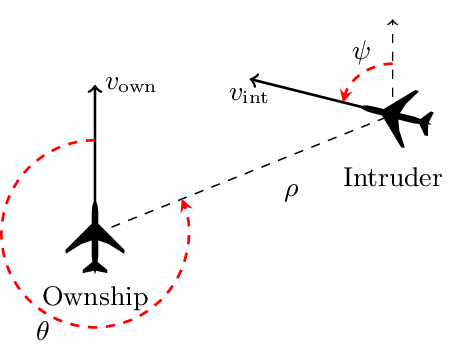
\includegraphics[width=0.5\linewidth]{img/acas_xu.png}};
}

\vspace{-1em}

Inputs:
\begin{itemize}
\setlength\itemsep{-0.1em}
\item Distance to intruder, $\rho$
\item Angle to intruder, $\theta$
\item Intruder heading, $\varphi$
\item Speed, $v_{own}$
\item Intruder speed, $v_{int}$
\end{itemize}

Outputs:
\begin{itemize}
\setlength\itemsep{-0.1em}
\item Clear of conflict
\item Strong left
\item Weak left
\item Weak right
\item Strong right
\end{itemize}

\end{frame}


\begin{frame}
\frametitle{ACAS Xu}

\begin{definition}[ACAS Xu: Property 3]
{\it If the intruder is directly ahead and is moving towards the
 ownship, the score for COC will not be minimal.}
\end{definition}

\begin{equation*}
\begin{array}{c}
1500 \leq \rho \leq 1800 \ \wedge -0.06 \leq \theta \leq 0.06 \ \wedge \psi \geq 3.10 \ \wedge 
  v_{own} \geq 980 \ \wedge v_{int} \geq 960 \
  \\
  \Rightarrow \\
\qquad
\exists a \in \{SL,L,R,SR\}. f(\theta, \rho, \varphi, v_{own}, v_{int})_{COC} < f(\theta, \rho, \varphi, v_{own}, v_{int})_a
\end{array}
\end{equation*}

\end{frame}

%\section{Vehicle' Syntax}

\begin{frame}[fragile]
\frametitle{Types}
Let us build the ACAS Xu specification.

We start with types of input and output vectors, as well as types of ACAS Xu networks

\vspace{1em}

\begin{minted}[fontsize=\small]{haskell}
type InputVector = Vector Rat 5
type OutputVector = Vector Rat 5

@network
acasXu : InputVector -> OutputVector
\end{minted}

\vspace{1em}

The Vector type represents a mathematical vector, or in programming terms can be thought of as a fixed-length array.
\end{frame}


\begin{frame}[fragile]
\frametitle{Values}

Types for values are automatically inferred by \textbf{Vehicle}. For example, we can declare the number $\pi$ and its type will be inferred as rational:

\begin{minted}[fontsize=\small]{haskell}
pi = 3.141592
\end{minted}
\end{frame}


\begin{frame}[fragile]
\frametitle{Working with vectors}

\underline{Problem}: The trained ACAS Xu network assumes that the inputs and outputs are normalised to values (roughly) between -2 and 2.

\pause
\vspace{1em}

However, we want to write our specifications over the original units! (e.g. $m/s$)

\pause
\vspace{1em}

This is an instance of the common \emph{problem space / input space mismatch}

\pause
\vspace{1em}

Being able to write specifications about the problem space is a feature that distinguishes \textbf{Vehicle} from
other neural network verifiers platforms.
\end{frame}

\begin{frame}[fragile]
\frametitle{Vector normalisation}
\vspace{-2em}
For clarity, we define a new type synonym for unnormalised input vectors which are in the problem space.
\begin{minted}[fontsize=\footnotesize]{haskell}

type UnnormalisedInputVector = Vector Rat 5

\end{minted}

Next we define the range of the inputs that the network is designed
to work over.

\begin{minted}[fontsize=\footnotesize]{haskell}

minimumInputValues : UnnormalisedInputVector
minimumInputValues = [0.0, -pi , -pi , 100.0, 0.0]

maximumInputValues : UnnormalisedInputVector
maximumInputValues = [60261.0, pi, pi, 1200.0, 1200.0]

meanScalingValues : UnnormalisedInputVector
meanScalingValues = [19791.091, 0.0, 0.0, 650.0, 600.0]
\end{minted}
\end{frame}



\begin{frame}[fragile]
\frametitle{Vector manipulation}
\vspace{-2em}
An alternative method to vector definition is to use the `foreach` constructor, which is used to provide a value for each `index i`.
\begin{minted}[fontsize=\footnotesize]{haskell}

minimumInputValues : UnnormalisedInputVector
minimumInputValues = foreach i . 0

\end{minted}
Let us see how  `foreach` works with vector indexing.

We can now define the normalisation function that takes an input vector and
returns the unnormalised version.

\begin{minted}[fontsize=\footnotesize]{haskell}

normalise : UnnormalisedInputVector -> InputVector
normalise x = foreach i .
  (x ! i - meanScalingValues ! i) / (maximumInputValues ! i)
\end{minted}

\pause
... our first acquaintance with functions!

\end{frame}



\begin{frame}[fragile]
\frametitle{Functions and types}
\begin{minted}[fontsize=\footnotesize]{haskell}
<name> : <type>
<name> [<args>] = <expr>

\end{minted}
Functions make up the backbone of the \textbf{Vehicle} language.
\pause
\begin{minted}[fontsize=\footnotesize]{haskell}

validInput : UnnormalisedInputVector -> Bool
validInput x = forall i .
  minimumInputValues ! i <= x ! i <= maximumInputValues ! i

\end{minted}

\pause

\begin{block}{Our first acquaintance with predicates and quantifiers!}
 One of the main advantages of \textbf{Vehicle} is that it can be used to state and prove specifications that describe the network’s behaviour over an infinite set of values.
\end{block}

\end{frame}



\begin{frame}[fragile]
\frametitle{Functions and types}

\begin{block}{Function Composition: Exercise}

What are the types of functions `acasXu`  and `normalise`:

\begin{minted}[fontsize=\footnotesize]{haskell}
normAcasXu : UnnormalisedInputVector -> OutputVector
normAcasXu x = acasXu (normalise x)
\end{minted}
\end{block}

\end{frame}

\begin{frame}[fragile]
\frametitle{Pre-defined functions and predicates}
We have already used:
\begin{minted}[fontsize=\footnotesize]{haskell}
*
/
!
<=
\end{minted}

\begin{block}{Exercise}
\footnotesize{What do they stand for?}
\end{block}
\end{frame}



\begin{frame}[fragile]
\frametitle{Let's verify ACAS Xu!}
\begin{minted}[fontsize=\footnotesize]{haskell}
distanceToIntruder = 0   -- measured in metres
angleToIntruder    = 1   -- measured in radians
intruderHeading    = 2   -- measured in radians
speed              = 3   -- measured in metres/second
intruderSpeed      = 4   -- measured in meters/second

clearOfConflict = 0
weakLeft        = 1
weakRight       = 2
strongLeft      = 3
strongRight     = 4
\end{minted}
\footnotesize{
The fact that all vector types come annotated with their size means that it
 is impossible to mess up indexing into vectors, e.g. if you changed
 `distanceToIntruder = 0` to `distanceToIntruder = 5` the specification would
 fail to type-check.}



\end{frame}

\begin{frame}[fragile]
\frametitle{Property 3}


\footnotesize{\textbf{If the intruder is \emph{directly ahead} and is moving towards the
 ownship, the score for COC will not be minimal.}}

\pause

\begin{minted}[fontsize=\footnotesize]{haskell}
directlyAhead : UnnormalisedInputVector -> Bool
directlyAhead x =
  1500  <= x ! distanceToIntruder <= 1800 and
  -0.06 <= x ! angleToIntruder    <= 0.06
\end{minted}
\pause
\begin{block}{Exercise!}
\footnotesize{
\begin{enumerate}
\item
Can you identify whether the specification is written in terms of input space or problem space? How do you know?
%\item Can you spot another pre-defined \textbf{Vehicle} function? What is it?
\end{enumerate}}
\end{block}

\end{frame}




\begin{frame}[fragile]
\frametitle{Property 3}

\footnotesize{\textbf{If the intruder is directly ahead and is \emph{moving towards} the
 ownship, the score for COC will not be minimal.}}

\pause

\begin{minted}[fontsize=\footnotesize]{haskell}
movingTowards : UnnormalisedInputVector -> Bool
movingTowards x =
  x ! intruderHeading >= 3.10  and
  x ! speed           >= 980   and
  x ! intruderSpeed   >= 960
\end{minted}


\end{frame}

\begin{frame}[fragile]
\frametitle{There is little left to do!}

\footnotesize{
\textbf{If the intruder is directly ahead and is moving towards the
 ownship, the \emph{score for COC will not be minimal}.}}

\pause

\begin{minted}[fontsize=\footnotesize]{haskell}
minimalScore : Index 5 -> UnnormalisedInputVector -> Bool
minimalScore i x =
   forall j . i != j => normAcasXu x ! i < normAcasXu x ! j
\end{minted}
\pause
\begin{block}{Exercise!}
\footnotesize{
\begin{enumerate}
\item What kind of domain  `forall` ranges over? Is it finite or infinite?
\end{enumerate}}
\end{block}

\end{frame}


\begin{frame}[fragile]
\frametitle{There is little left to do!}

\footnotesize{
\textbf{If the intruder is directly ahead and is moving towards the
 ownship, the score for COC will not be minimal.}}

\pause

\begin{minted}[fontsize=\footnotesize]{haskell}
@property
property3 : Bool
property3 = forall x . validInput x and
                       directlyAhead x and
                       movingTowards x =>
                       not (minimalScore clearOfConflict x)
\end{minted}
\pause
\begin{block}{Exercise!}
\footnotesize{
\begin{enumerate}
\item Can you guess the purpose of the `@property` syntax?
\item What kind of domain  `forall` ranges over? Is it finite or infinite?
\end{enumerate}}
\end{block}

\end{frame}



\begin{frame}[fragile]
\frametitle{How to run Vehicle}
\vspace{-2em}
\begin{block}{Checklist}
\begin{enumerate}
\item Vehicle and Marabou are installed.
\item navigate to \texttt{examples/chapter2/acasXu} in the tutorial repo.
\end{enumerate}
\end{block}

\pause
\begin{minted}[fontsize=\footnotesize]{haskell}
vehicle verify \
  --specification acasXu.vcl \
  --verifier Marabou \
  --network acasXu:acasXu_1_7.onnx \
  --property property3

Verifying properties:
property3 [==========================================] 1/1 queries
  result:  counterexample found
  x: [1799.9886669999978, 1.9509286320000003e-2,
                        3.09999732192, 980.0, 1017.6036]
\end{minted}
\end{frame}




\begin{frame}
\frametitle{Verifier limitations}

Vehicle is very expressive... \pause but most verifiers can only solve \textbf{linear} specifications with \textbf{non-alternating quantifiers}.

\pause
\vspace{1em}

What does Vehicle do when you write such a specification?
\end{frame}


\begin{frame}
\frametitle{Use the type-checker over and over...}

\newcommand{\typebox}{aisecyellow}

\begin{tikzpicture}
\node (start) at (-1.5,3) {};

\node[rectangle,draw] (scope) at (0,3) {\textbf{Scoping}};

\node[rectangle,draw, fill=\typebox] (type) at (2.5,3) {\textbf{Type check}};

\node[rectangle,draw] (normalise) at (6.5,3) {\textbf{Normalise}};

\node[rectangle,draw] (queries) at (9,3) {\textbf{Queries}};

\node(endqueries) at (11.5,3) {Marabou};

\draw [->] (start) edge (scope);
\draw [->] (scope) edge (type);
\draw [->] (type) edge node [above]{verifiers} (normalise);
\draw [->] (normalise) edge (queries);
\draw [->] (queries) edge (endqueries);

%% Linearity errors

\onslide<3->{
\node[rectangle,draw, fill=aisecred!50] (linerror) at (5,4.5) {\textbf{Linearity error}};

\node[rectangle, fill=\typebox, draw, text width=2cm, align=center] (lintype) at (8.2,4.5) {\textbf{Linearity type check}};

\node[rectangle,draw,text width=2cm, align=center] (linmessage) at (11,4.5) {\textbf{Error message}};

\draw [->] (normalise) edge (linerror);
\draw [->] (linerror) edge (lintype);
\draw [->] (lintype) edge (linmessage);
}

%% Polarity errors

\onslide<4->{
\node[rectangle,draw,fill=aisecred!50] (polerror) at (5,1.5) {\textbf{Quantifier error}};

\node[rectangle, fill=\typebox, draw,text width=2cm, align=center] (poltype) at (8.2,1.5) {\textbf{Quantifier type check}};

\node[rectangle,draw,text width=2cm, align=center] (polmessage) at (11,1.5) {\textbf{Error message}};

\draw [->] (normalise) edge (polerror);
\draw [->] (polerror) edge (poltype);
\draw [->] (poltype) edge (polmessage);
}

%% Training

\onslide<5->{
\node[rectangle, fill=\typebox, draw,text width=2.5cm, align=center] (difftype) at (1.5,5) {\textbf{Differentiable type check}};

\node[rectangle,draw] (lossfunc) at (5,5.5) {\textbf{Loss function}};

\node (endloss) at (11.2,5.5) {Tensorflow};

\draw [->] (type) edge node [left]{training} (difftype);
\draw [->] (difftype) edge (lossfunc);
\draw [->] (lossfunc) edge (endloss);
}

%% Agda

\onslide<6->{
\node[rectangle, fill=\typebox, draw,text width=2.5cm, align=center] (booltype) at (1.5,1) {\textbf{Bool/Set type check}};

\node[rectangle,draw] (agdacode) at (5,0.5) {\textbf{Agda code}};

\node (endagda) at (11.8,0.5) {Agda};

\draw [->] (type) edge node [left]{export} (booltype);
\draw [->] (booltype) edge (agdacode);
\draw [->] (agdacode) edge (endagda);

}
\end{tikzpicture}

\end{frame}

\begin{frame}
\frametitle{Secondary type systems...}

These secondary type-systems not possible without:
\begin{itemize}
\item A modular type-checker that is generic over the set of builtin types.

\item Backtracking instance search.

\item Automatic generalisation over unsolved metas and instance constraints.

\item Dependent types (for operations over provenance information stored in the types).
\end{itemize}

\vspace{2em}
\pause

The user is expected to make very little use of these features!

\end{frame}


\begin{frame}
\frametitle{What we've seen in this chapter ...}

\vspace{-1em}

\begin{center}
\begin{tikzpicture}[thick,
    set/.style = {circle,
        minimum size = 3cm}]

% Set A
\node[rectangle,draw] (A) at (1.5,5) {\alert{\textbf{Property in Vehicle}}};

\node[rectangle,draw] (B) at (-3,2) {Training};
\node[text width=1cm, align=center] at (-3,0) {DL2 ACT etc.};

\node[rectangle,draw, dashed, text width=1.4cm] (C) at (0,2) {Counter-example search};
\node[text width=1cm, align=center] at (0,0) {PGD FGSM etc.};

\node[rectangle,draw] (D) at (3,2) {\alert{\textbf{Verification}}};
\node[text width=1.4cm, align=center] at (3,0) {\alert{\textbf{Marabou}} Eran etc.};

\node[rectangle,draw] (E) at (6,2) {Integration};
\node[text width=2cm, align=center] at (6,0) {Agda, Coq, KeymaeraX etc.};

\draw [->] (A) edge (B);
\draw [->, dashed] (A) edge (C);
\draw [->] (A) edge (D);
\draw [->] (A) edge (E);

\draw [->] (B) edge (C);
\draw [->] (C) edge (D);
\draw [->] (D) edge (E);

\onslide<1->{
\node[rectangle,draw,fill=normal text.bg] (D) at (1.5,4) {\alert{\textbf{Analysis \& informative error messages}}};
}

\end{tikzpicture}
\end{center}
\end{frame}




\begin{frame}
\frametitle{Concluding Exercise}

Which of the four PL problems we addressed?

\begin{itemize}
\item[$I^O$] Interoperability -- properties are not portable between training/counter-example search/ verification.

\item[$I^{P}$] Interpretability -- code is not easy to understand.

\item[$I^{\int}$] Integration -- properties of networks cannot be linked to larger control system properties.

\item[$E^G$] Embedding gap -- little support for translation between problem space  and input space.
\end{itemize}
\end{frame}


\begin{frame}
\frametitle{Harder Exercise: ACAS Xu Property 1}
\vspace{-2em}
ACAS Xu Property 1 gives an idea how the {\it embedding gap}
 can arise not only when we reason about inputs, but also  the outputs of networks!
%In the previous lecture, we introduced ACAS Xu property 1.


\pause

\begin{definition}[ACAS Xu: Property 1]
\small{\it If the intruder is distant and is significantly slower than the ownship, the score of a COC advisory will always be below a certain fixed threshold:}

\begin{equation*}
\begin{array}{l}
(\rho \geq 55947.691) \wedge
(v_{own} \geq 1145) \wedge (v_{int} \leq 60)  \\
\Rightarrow \text{the score for COC is at most } 1500
\end{array}
\end{equation*}
where the neural network outputs are scaled as follows: given an element $x$ of the output vector, we scale it as: $\frac{x - 7.518884}{373.94992}$.

\pause


\end{definition}

\begin{itemize}
\item Can you formalise Property 1 in Vehicle?
\item Can you spot the embedding gap, this time concerning the network's output?
\end{itemize}
\end{frame}

\end{document}


\begin{frame}[fragile]
\frametitle{Next Lecture: $\epsilon$-ball Robustness}
 \begin{minted}[fontsize=\tiny]{haskell}
type Image = Tensor Rat [28, 28]
type Label = Index 10
validImage : Image -> Bool
validImage x = forall i j . 0 <= x ! i ! j <= 1

@network
classifier : Image -> Vector Rat 10

advises : Image -> Label -> Bool
advises x i = forall j . j != i => classifier x ! i > classifier x ! j

@parameter
epsilon : Rat

boundedByEpsilon : Image -> Bool
boundedByEpsilon x = forall i j . -epsilon <= x ! i ! j <= epsilon

robustAround : Image -> Label -> Bool
robustAround image label = forall pertubation .
  let perturbedImage = image - pertubation in
  boundedByEpsilon pertubation and validImage perturbedImage =>
    advises perturbedImage label

@dataset
trainingImages : Vector Image n

@dataset
trainingLabels : Vector Label n

@property
robust : Vector Bool n
robust = foreach i . robustAround (trainingImages ! i) (trainingLabels ! i)
\end{minted}
\end{frame}


\begin{frame}
\frametitle{Plan for the rest of this tutorial}

\begin{itemize}
\item Before coffee break:
\begin{itemize}
%\item Brief introduction to \textbf{Vehicle} specification language
\item \alert{Exercise session:} write and verify your own specs (with possibility to extend over the break)

\begin{itemize}
\item for writing a spec, install vehicle: just run

\texttt{pip install vehicle-lang}

\item for verifying a spec, you also need Marabou installed

\texttt{pip install maraboupy}
\end{itemize}
\end{itemize}
\end{itemize}
\end{frame}


\begin{frame}
\frametitle{Exercises}

\begin{block}{Robustness (for those familiar with the problem)}
\footnotesize{
\begin{itemize}
\item Fill in missing code in the Robustness spec available at
\url{https://github.com/vehicle-lang/tutorial}:\\
\url{exercises/Chapter 2. Getting Started/mnist-robustness}

\item Using the given neworks and data, verify robustness via Vehicle.
\end{itemize}}
\end{block}

\begin{alertblock}{Robustness (for those NOT familiar with the problem)}
\footnotesize{Study the chapter ``Proving Neural Network Robustness" here: \url{https://vehicle-lang.github.io/tutorial/}}
\end{alertblock}

\begin{block}{More ACAS Xu properties in the same spec}
\footnotesize{
\begin{itemize}
\item Extend the given ACAS Xu  specification with Property 1.
The spec and network can be found at:
\url{https://github.com/vehicle-lang/tutorial}, at \\
\url{examples/Chapter 2. Getting Started/acasXu}
\item Using the given neworks and data, verify the properties via Vehicle.
\end{itemize}}
\end{block}

\end{frame}
\end{document}
